\section{ SR02NL23 }


\subsection{Meta}

    \textbf{Title:}
    Integrated Planning in Hospitals: A Review}

    \begin{table}[H]
        \centering
        \begin{tabular}{|c|c|c|c|c|c|c|c|c|}
            \hline
                \textbf{Rank} & \textbf{Grasp} & \textbf{Grade} & \textbf{Type} & \textbf{Outcome} & \textbf{Domain} & \textbf{COV19} & \textbf{CoI} & \textbf{DB} \\
            \hline
                5 & 96\% & A & A & P & B & Yes & ?? & No \\
            \hline
        \end{tabular}
        \caption{Reference's metadata}
        \label{tab:SR02NL23}
    \end{table}

\subsection{Summary}
    Sebastian Rachuba, Melanie Reuter-Oppermann, and Clemens Thielen conducted a literature review considering hospital-integrated planning. The authors rendered a standard systematic literature review with taxonomy analysis. By the author's narrative, integrated refers to the interconnection of hospital resources and the mutual influence of different aspects of healthcare related to medical care planning. The three levels of integration were defined, and among these three levels, the reviewed studies were distributed. The integration of hospital planning was discussed, including the hospital levels of strategy, planning approaches, research objectives, and connections between research criteria. The arguments were supported by graphical visualisation of the analysed data. The main conclusions of the work are that the trends are shifting toward medical stuff from operating theatres, and there is a possible increase in papers which investigate healthcare services with no direct interaction with patients, such as pharmacy and OT cleaning. 
    

\subsection{Notes}
    \begin{itemize}
        \item Health departments disconnection;
        \item Vertical/ horisontal integrated;
        \item \url{www.webofscience.com}
    \end{itemize}


\subsection{Reading}
    \textbf{Abstract:}
    This literature review is about an integrate operating theatre scheduling. The abstract begines with the starting point of medical resource scheduling in scientific literature which is year 1950. The work proposes a taxonomy analysis of the current state of operating theatre scheduling research.
    
    \textbf{Objectives:}
    Research the existing literature in scope of healthcare integrated planning.

    
    \textbf{Page 1:}
    The importance of healthcare system in modern world can be seen in the budgets issues for the healthcare need in Europ which is almost 11\%.
    
    \textbf{Page 2:}
    The ever increasing demand of the healthcare services can be regulated with the improvement of the medical resource management. One of the obsticles is disconnection between departments even in the same hospital. The efficient method to ensure interconnection between various departments is to use horizontal and vertical integrated in hospitals.
    
    \textbf{Page 3:}
    The structure of the paper as well as the methods used for searching the literature were outlined on this page.
    
    \textbf{Page 4:}
    The authors did not limit the approved for in-depth review papers by the year of publication. For the detailed review 318 potential studies were selected.
    
    \textbf{Page 5:}
    This page introduces the classification of the papers by their level of integrated. There are three levels of hospital planning integrated.
    \begin{figure}[H]
        \centering
        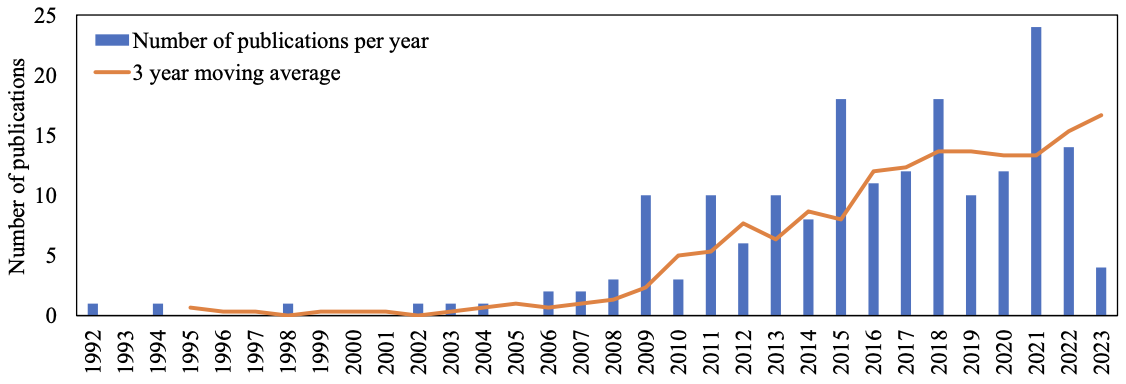
\includegraphics[width=1\textwidth]{figures/0010_SR02NL23/fig1.png}
        \caption{Number of publications over the years from \cite{x338}.}
        \label{fig1:0010_SR02NL23}
    \end{figure}
    
    \textbf{Page 6:}
    On this page, the authors explaine the connection between all three level of integrated and how does it interpreted into the operating theatre planning and scheduling.

    \textbf{Page 7:}
    The second level of integrated planning is the least investigated and the first and the third levels have been interchanbaly in the lead by number of publications from year to year. Another tendency is in the number of tactical and strategical planning. The hbroader the perspective the smaller number of papers have looked into this, and it is true for all three levels of integrated.
    
    \textbf{Page 8:}
    Here the authors list a medical resources that are objectives of the scheduling and planning.
    \begin{figure}[H]
        \centering
        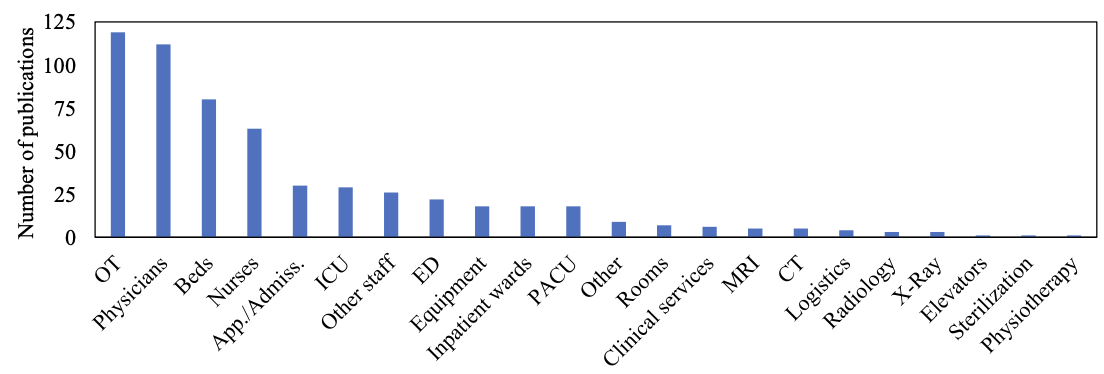
\includegraphics[width=1\textwidth]{figures/0010_SR02NL23/fig2.png}
        \caption{Objective trends in \cite{x338}.}
        \label{fig2:0010_SR02NL23}
    \end{figure}
    
    \textbf{Page 9:}
    Operating theatres are most ofteen considered as a promary resources.
    \begin{figure}[H]
        \centering
        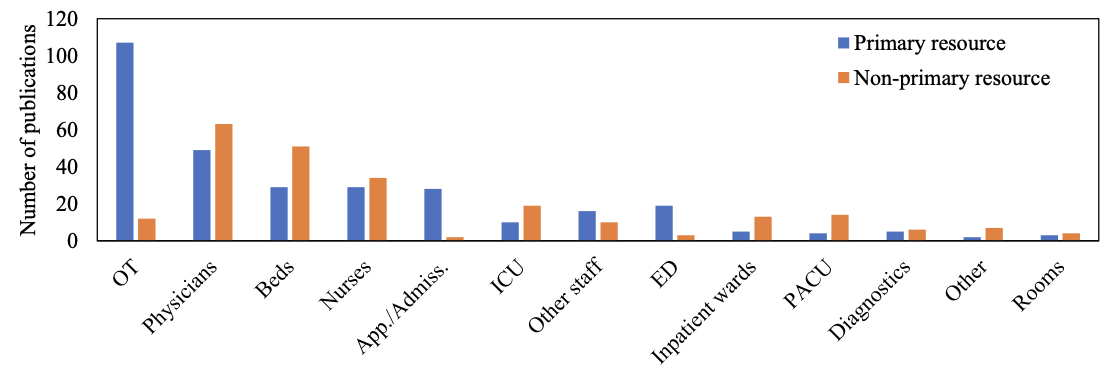
\includegraphics[width=1\textwidth]{figures/0010_SR02NL23/fig3.png}
        \caption{Objective trends as primary or secondary critaria in \cite{x338}.}
        \label{fig3:0010_SR02NL23}
    \end{figure}
    
    \textbf{Page 10:}
    The authors looked into the combinations of the resources in the literature.
    \begin{figure}[H]
        \centering
        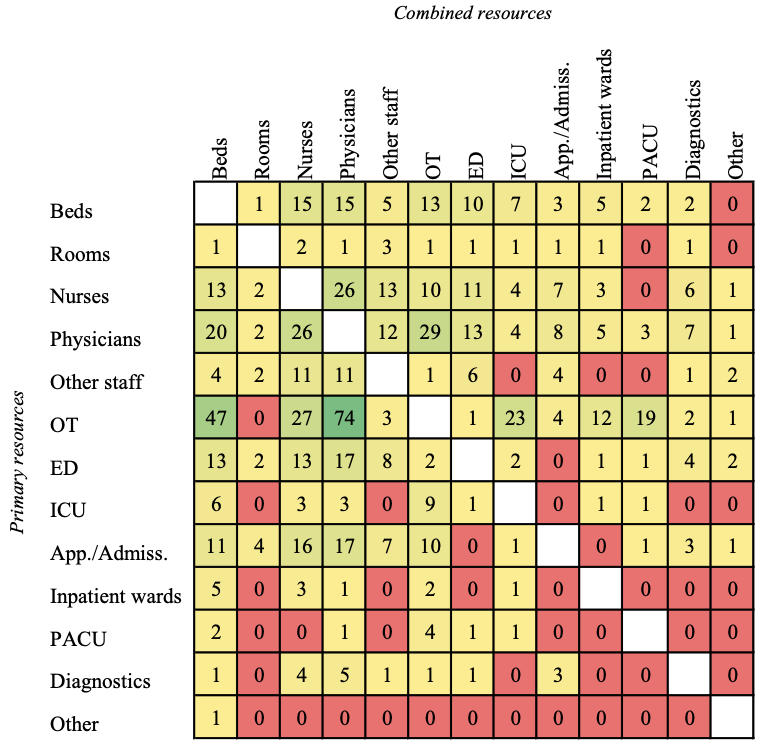
\includegraphics[width=1\textwidth]{figures/0010_SR02NL23/fig4.png}
        \caption{Resource combinations from \cite{x338}.}
        \label{fig4:0010_SR02NL23}
    \end{figure}

    \textbf{Page 11:}
    \begin{figure}[H]
        \centering
        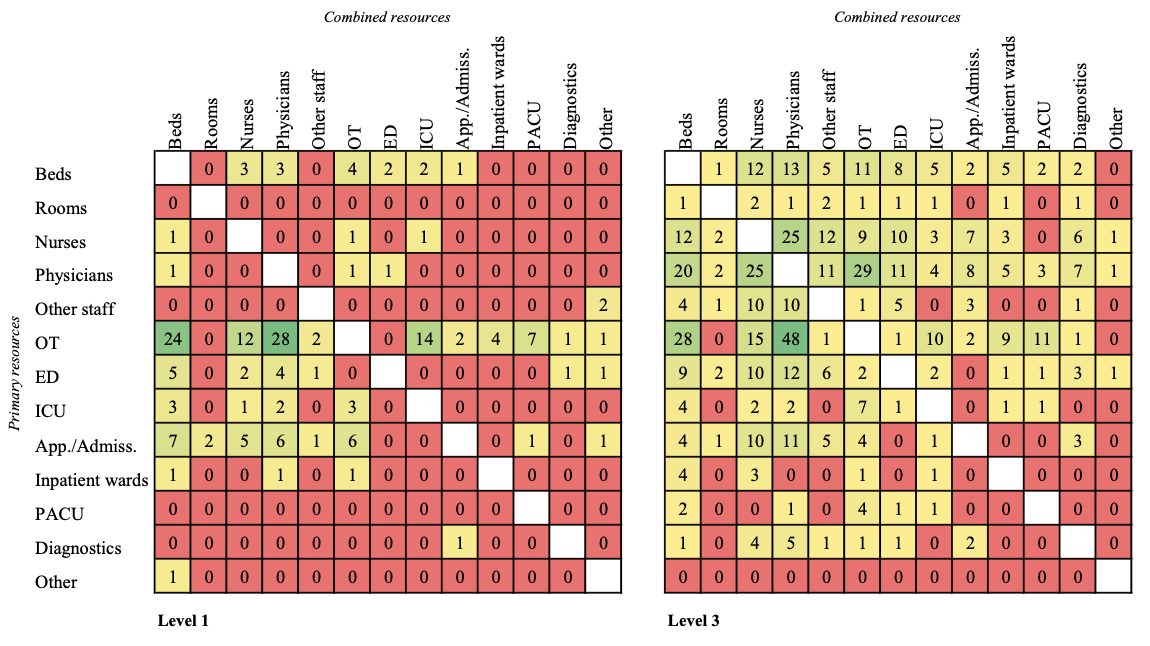
\includegraphics[width=1\textwidth]{figures/0010_SR02NL23/fig5.png}
        \caption{Resource combinations by livel of integraion planning from \cite{x338}.}
        \label{fig5:0010_SR02NL23}
    \end{figure}
    
    \textbf{Page 12:}
    Here was stated that the focus from OT planning and scheduling shifts toward the medical staff members with increasing of the integrity of the model. This page lists the solution approaches to the different levels of integrated planning. The combination of approaches gained its popularity amoung researchers.
    
    \textbf{Page 13:}
    The authors segment the planning solutions into three categoris: optimisations, symulations, and other. The flows of the number of publications amonng years have been provided.

    \textbf{Page 14:}
    One unexpected tendency is regarding stuff related planning and optimisation panning approaches. The optimisation methods are used less for stuff and more for all other objectives, where stuff related problems are usually solved by simulations or other methods.
    \begin{figure}[H]
        \centering
        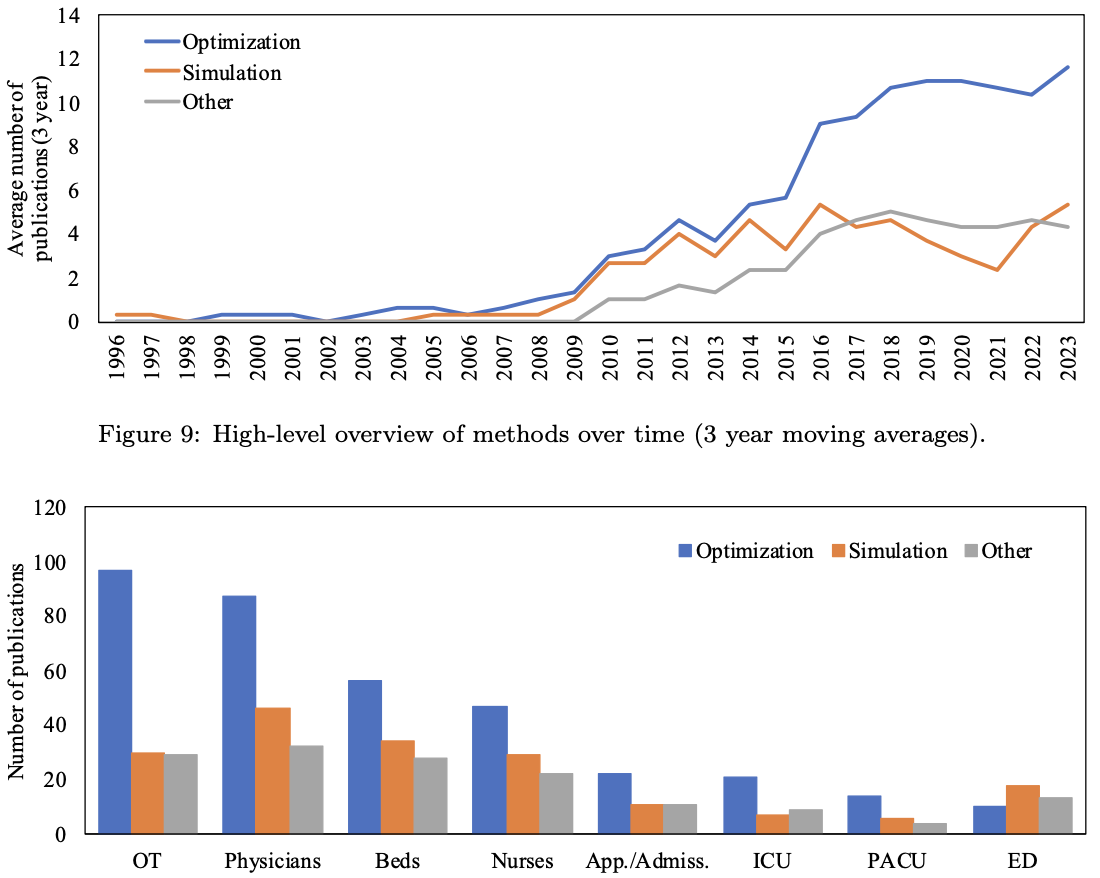
\includegraphics[width=1\textwidth]{figures/0010_SR02NL23/fig6.png}
        \caption{Publication trends between 1996 and 2023 from \cite{x338}.}
        \label{fig6:0010_SR02NL23}
    \end{figure}

    \textbf{Page 15:}
    In this page more in-depth analysis of the trends in relation to levels of integrated was conducted.
    
    \textbf{Page 16:}
    Here is the final thought about general features of the studies, and the analysis continues to a practical side of the medical resource scheduling and planning which consideres uncertanties.
    
    \textbf{Page 17:}
    More analysis regarding the models with uncertainties.
    \begin{figure}[H]
        \centering
        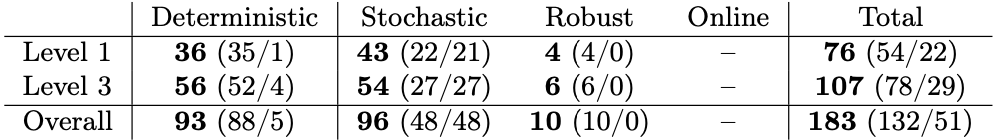
\includegraphics[width=1\textwidth]{figures/0010_SR02NL23/fig7.png}
        \caption{Studies that considered deterministic, stochastic, robust, and online in relation to the level of integrated in \cite{x338}.}
        \label{fig7:0010_SR02NL23}
    \end{figure}

    \textbf{Page 18:}
    The reviewved works offer a veriaty of different uncertainties in the healthcare envorenment. Only a minority of the reviewed studies implement their models into real hospitals. Thera also other approaches to evaluate the developed scheduling approach.

    \textbf{Page 19:}
    Basically in this page tha authors describe the chart below ephacising that the are not many practical implementations of research, which indicates that journal publishers does not care about this aspect too much.
    \begin{figure}[H]
        \centering
        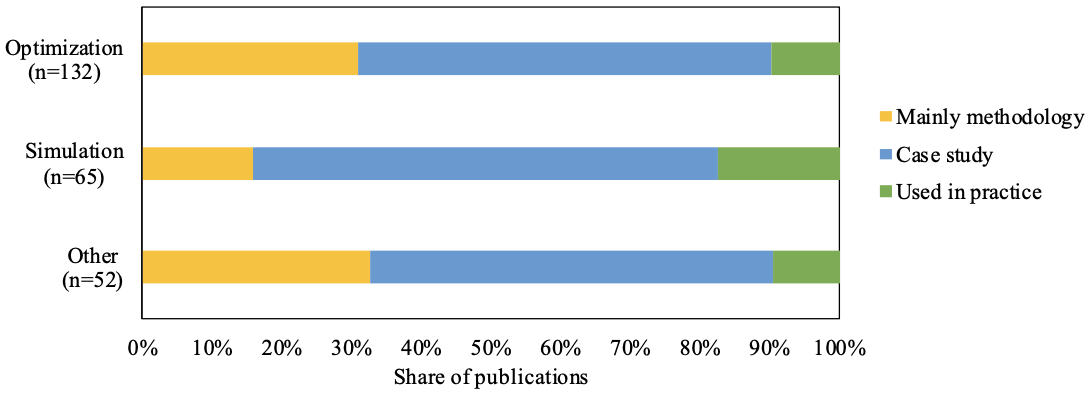
\includegraphics[width=1\textwidth]{figures/0010_SR02NL23/fig8.png}
        \caption{Distribution of theoretical work, case study, and implemented research for optimisations, simulations, and other approaches in \cite{x338}.}
        \label{fig8:0010_SR02NL23}
    \end{figure}
    
    \textbf{Page 20:}
    Here is an introduction of three departments depend on the patient stage of the healthcare flow: pre-hospital departments, during-hospital departments, and post-hospital departments.
    
    \textbf{Page 21:}
    The department interconnections.
    \begin{figure}[H]
        \centering
        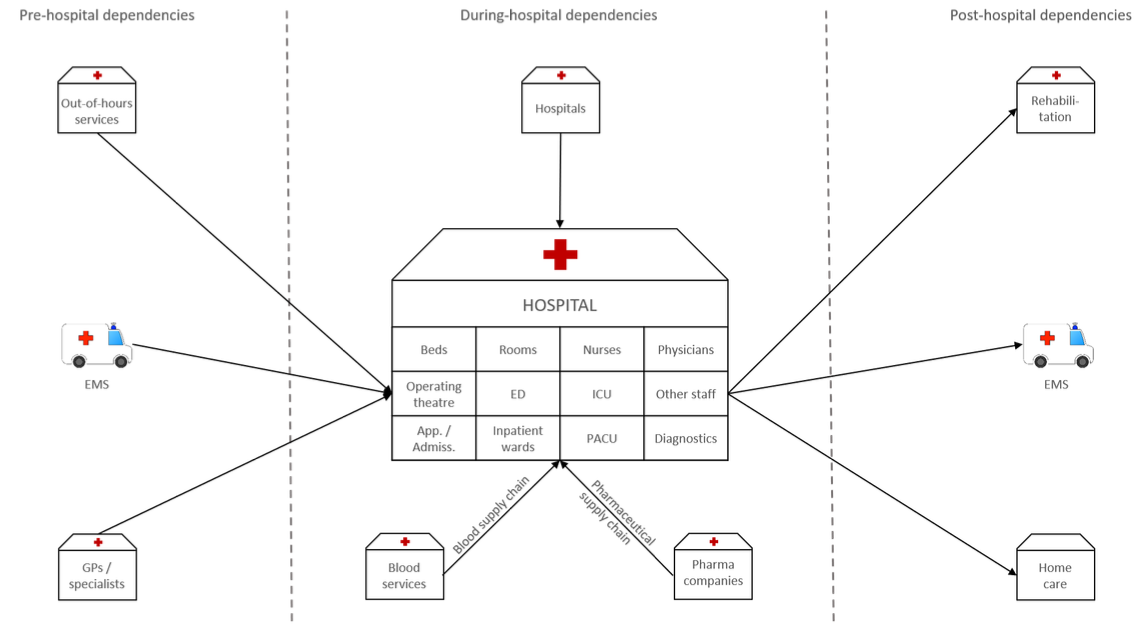
\includegraphics[width=1\textwidth]{figures/0010_SR02NL23/fig9.png}
        \caption{Hospital departments from \cite{x338}.}
        \label{fig9:0010_SR02NL23}
    \end{figure}
    
    \textbf{Page 22:}
    The main resources in during-hospital department and bottlnecks in post-hospital demartments were discussed on this page.
    
    \textbf{Page 23:}
    The trends show that if consider nurses and phisicians ander one term medical staff the number of publications starting from 2010 exceeds the number of publivations for OT. Nevertheless, OT still remains the most frequently considered primary objective in the medical resource scheduling research.
    
    \textbf{Page 24:}
    There is still lack in studies which condidering uncertainties. Tha authors predict that it possibly will change in the near future, because the number of related work is growing. Implementation of the research findings on practice is also not frequent fenomena.
    \begin{figure}[H]
        \centering
        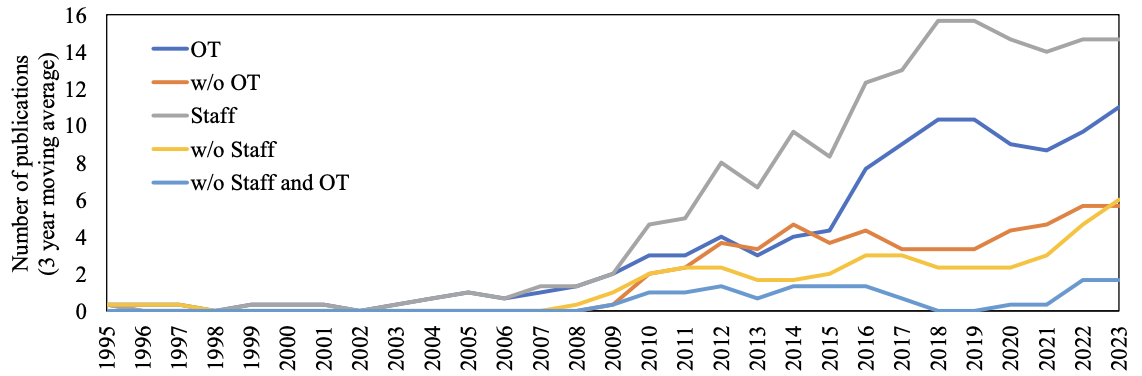
\includegraphics[width=1\textwidth]{figures/0010_SR02NL23/fig10.png}
        \caption{3-year moving averages of the numbers of publications that do / do not consider OT or medical staff. from \cite{x338}.}
        \label{fig10:0010_SR02NL23}
    \end{figure}

    \textbf{Page 25:}
    The ephasis in the research gap lies on studies wich do not interact with the patient directly (pharmacy for instance) and also onto medical staff oriented research.

    \textbf{Page 26:}
        1. Planning which does not involve patients diractly; 2. Medical staff choreography; 3. Simulation studies; 4. Practical implementations.